\documentclass[11pt,a4paper]{article}
\usepackage[margin=23mm]{geometry}
\usepackage[T1]{fontenc}\usepackage[utf8]{inputenc}\usepackage{lmodern,microtype}
\usepackage{amsmath,amssymb,bm,booktabs,longtable,array,graphicx,float}
\usepackage[dvipsnames]{xcolor}\usepackage{tikz}\usetikzlibrary{arrows.meta,calc,positioning,decorations.pathmorphing,shapes.geometric}
\usepackage[most]{tcolorbox}\usepackage{enumitem,fancyhdr,lastpage}
\usepackage[colorlinks=true,linkcolor=MidnightBlue,urlcolor=MidnightBlue]{hyperref}
\hypersetup{pdftitle={The Physics Behind Pendulum Game},pdfauthor={Pendulum Game technical guide},pdfsubject={Beginner-friendly explanation of the v0.1.0 simulation},pdfkeywords={pendulum, physics, RK4, Lagrangian mechanics, game simulation}}
\definecolor{teal}{HTML}{147A88}\definecolor{ink}{HTML}{19354A}\definecolor{warm}{HTML}{B95C24}
\setlength{\parindent}{0pt}\setlength{\parskip}{6pt}\linespread{1.08}
\setlist{nosep,topsep=5pt,leftmargin=*}
\pagestyle{fancy}\fancyhf{}\fancyhead[L]{\small Pendulum Game: Physics Explained}\fancyhead[R]{\small v0.1.0}\fancyfoot[C]{\thepage\ / \pageref{LastPage}}
\setlength{\headheight}{14pt}
\newtcolorbox{idea}[1]{colback=teal!5,colframe=teal,title=#1,fonttitle=\bfseries}
\newtcolorbox{arcade}{colback=orange!5,colframe=warm,title=Physical model or arcade rule?,fonttitle=\bfseries}
\newcommand{\code}[1]{\texttt{\detokenize{#1}}}
\newcommand{\dd}{\mathrm{d}}\newcommand{\vect}[1]{\boldsymbol{#1}}
\tikzset{rod/.style={line width=2.2pt,ink},mass/.style={circle,draw=ink,fill=teal!30,minimum size=9mm},arr/.style={-{Latex[length=2.5mm]},thick},ghost/.style={dashed,gray},target/.style={circle,draw=red!70!black,fill=red!15,minimum size=9mm},every node/.style={font=\small}}
\title{\Huge\bfseries The Physics Behind\\Pendulum Game\\[8mm]\Large A beginner-friendly guide to the actual simulation}
\author{Technical explanation of the v0.1.0 implementation}
\date{31 October 2026}
\begin{document}
\begin{titlepage}\maketitle\thispagestyle{empty}
\begin{center}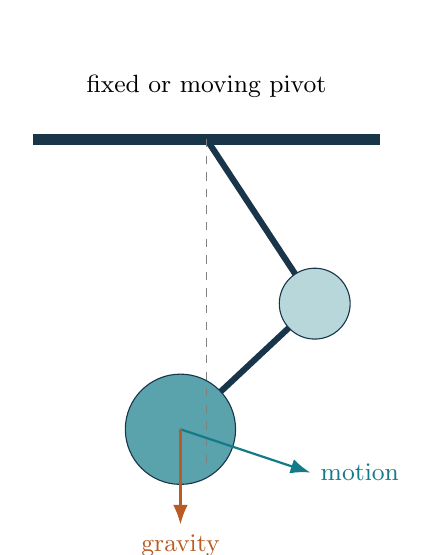
\begin{tikzpicture}[scale=1.1]
\draw[ink,line width=4pt](-2,0)--(2,0);\coordinate(P)at(0,0);\coordinate(A)at(1.25,-1.9);\coordinate(B)at(-.3,-3.35);\draw[rod](P)--(A)--(B);\node[mass]at(A){};\node[mass,fill=teal!70,minimum size=14mm]at(B){};\draw[ghost](P)--(0,-3.8);\draw[arr,teal](B)--++(1.5,-.5)node[right]{motion};\draw[arr,warm](B)--++(0,-1.1)node[below]{gravity};\node[above=4mm]at(P){fixed or moving pivot};
\end{tikzpicture}\end{center}
\vfill
\begin{idea}{What you will learn}
Why the bob swings; how several links influence each other; how launch settings, gravity, wind and moving anchors change motion; how the computer advances time; and how targets, bombs, bumpers, portals, lasers and other gimmicks interact with the simulation.
\end{idea}
\textbf{Source baseline:} release tag \code{v0.1.0}, commit \code{6335b08}. This document describes that code, not an idealized replacement. Mathematics is introduced gradually; the derivation and source map provide a deeper reference.
\end{titlepage}
\setcounter{tocdepth}{1}
\tableofcontents\clearpage

\section{Start with the objects you see}
A pendulum is a mass that can swing around a support. In a simple classroom example, a weight hangs from a string. In this game, straight links join several masses. The final mass is called the \emph{tip bob}. The support at the beginning of the chain is the \emph{pivot} or anchor.

The links constrain where the masses can move. A bob cannot travel freely in a straight line while its link remains attached: its motion must also satisfy the link length. Two or more links create a much richer set of possible positions.
\begin{figure}[H]\centering
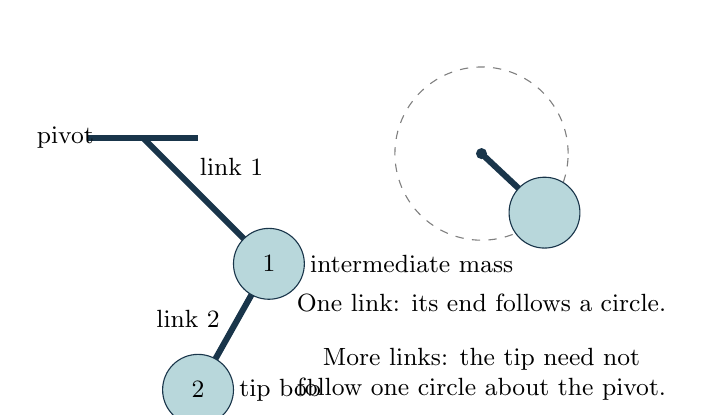
\begin{tikzpicture}
\coordinate(P)at(0,0);\coordinate(A)at(1.6,-1.6);\coordinate(B)at(.7,-3.2);
\draw[rod](-.7,0)--(.7,0);\draw[rod](P)--(A)--(B);\node[mass]at(A){1};\node[mass]at(B){2};
\node[left=5mm]at(P){pivot};\node[right=4mm]at(A){intermediate mass};\node[right=4mm]at(B){tip bob};\node[above right]at(.6,-.6){link 1};\node[left]at(1.1,-2.3){link 2};
\draw[ghost](4.3,-.2)circle(1.1);\fill[ink](4.3,-.2)circle(2pt);\draw[rod](4.3,-.2)--(5.1,-.95);\node[mass]at(5.1,-.95){};\node[align=center]at(4.3,-2.1){One link: its end follows a circle.};\node[align=center]at(4.3,-3){More links: the tip need not\\follow one circle about the pivot.};
\end{tikzpicture}
\caption{The support, links and masses. The code models massless rigid links and point masses for the equations of motion. Visible bob radii are used separately for contact tests.}
\end{figure}
\subsection{The model's assumptions}
The main simulation uses the following simplifications:
\begin{itemize}
\item Motion is two-dimensional: all movement stays in the screen's plane.
\item Links have fixed lengths and no modeled mass. They can push or pull like rigid rods; they are not slack strings.
\item Mass is concentrated at each joint. Standard gameplay initializes every mass to the same value, \(m_i=1\) in model units.
\item Joints do not have angle stops. Links can rotate through full turns and can pass through each other; rod--rod contact is not solved.
\item Ordinary stage chains have a total length of \(2.5\) model length units, divided evenly across the chosen number of links.
\end{itemize}
\begin{arcade}The artwork shows thick rods and round, growing bobs. The dynamics do not treat them as spinning solid rods or spheres. In particular, making the visible bob larger does \emph{not} change its mass or the mass matrix.\end{arcade}

\section{A short mathematical toolkit}
\subsection{Position, velocity and acceleration}
\textbf{Position} tells us where an object is. \textbf{Velocity} tells us how fast its position changes and in which direction. \textbf{Acceleration} tells us how its velocity changes. Acceleration can turn motion as well as speed it up or slow it down.

For a horizontal coordinate \(x\), the notation
\[
 v_x=\frac{\dd x}{\dd t}=\dot x,\qquad a_x=\frac{\dd v_x}{\dd t}=\ddot x
\]
means ``change of \(x\) per second'' and ``change of \(v_x\) per second.'' A dot means a time derivative; it is not multiplication. You can read these expressions as definitions even without studying calculus.

An angle has similar quantities: \(\theta\) is angle, \(\omega=\dot\theta\) is angular velocity, and \(\alpha=\dot\omega\) is angular acceleration. A negative angular velocity means rotation in the negative-angle direction, not negative speed. The speed magnitude is nonnegative.
\subsection{Degrees and radians}
The angle slider uses degrees. The solver uses radians:
\[
 \theta_{\mathrm{rad}}=\theta_{\mathrm{deg}}\frac{\pi}{180},\qquad
 180^\circ=\pi\ \mathrm{rad}.
\]
A radian measures arc length divided by radius. A complete turn is \(2\pi\) radians. The initial-angular-velocity slider is used directly as radians per model second; it is not converted from degrees per second.
\subsection{Vectors, sine and cosine}
A two-dimensional vector is an ordered pair, such as \(\vect v=(v_x,v_y)\). Its length is \(\lVert\vect v\rVert=\sqrt{v_x^2+v_y^2}\). Sine and cosine resolve a link into horizontal and vertical pieces. A dot product, \(\vect a\cdot\vect b=a_xb_x+a_yb_y\), measures how much one direction lines up with another.
\begin{idea}{Useful units}
Lengths in the solver are model metres, time is measured in seconds, \(\omega\) is in rad/s, and acceleration is in model m/s\(^2\). These are consistent modeling conventions, not a claim that the screen shows a literal full-size laboratory apparatus. Pixels are converted separately.
\end{idea}

\section{Coordinates: why the game uses sine for horizontal position}
The screen's \(x\)-axis points right and its \(y\)-axis points down. The angle \(\theta=0\) means a link hangs vertically downward. Positive angles lean right from that downward direction.
\begin{figure}[H]\centering
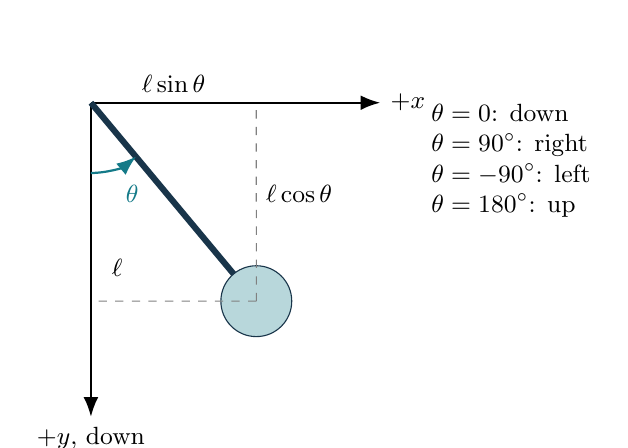
\begin{tikzpicture}[scale=1.05]
\coordinate(P)at(0,0);\coordinate(B)at(2,-2.4);\draw[arr](P)--(3.5,0)node[right]{\(+x\)};\draw[arr](P)--(0,-3.8)node[below]{\(+y\), down};\draw[rod](P)--(B);\node[mass]at(B){};\draw[ghost](B)--(0,-2.4);\draw[ghost](B)--(2,0);\draw[arr,teal](0,-.85)arc[start angle=-90,end angle=-50,radius=.85];\node[teal]at(.5,-1.1){\(\theta\)};\node[above]at(1,0){\(\ell\sin\theta\)};\node[right]at(2,-1.1){\(\ell\cos\theta\)};\node[left]at(.5,-2){\(\ell\)};
\node[align=left,anchor=west]at(4,-.7){\(\theta=0\): down\\\(\theta=90^\circ\): right\\\(\theta=-90^\circ\): left\\\(\theta=180^\circ\): up};
\end{tikzpicture}
\caption{The screen convention. The vertical component is positive downward, unlike many textbook diagrams.}
\end{figure}
For one link of length \(\ell\) and pivot \((x_p,y_p)\),
\begin{equation}\label{eq:position1}x=x_p+\ell\sin\theta,\qquad y=y_p+\ell\cos\theta.\end{equation}
For mass \(k\) on a chain, add the displacement of every link before it:
\begin{equation}\label{eq:positionN}
x_k=x_p+\sum_{i=1}^{k}\ell_i\sin\theta_i,\qquad y_k=y_p+\sum_{i=1}^{k}\ell_i\cos\theta_i.
\end{equation}
\textbf{Every \(\theta_i\) is an absolute angle from vertical.} Link 2's stored angle is not an angle relative to link 1. This distinction matters when interpreting the state array and portal calculations.

The standard canvas is \(800\times600\) pixels with base pivot \((400,300)\). The factor \(s=120\) pixels per model metre converts every length in equations~\eqref{eq:position1}--\eqref{eq:positionN} to drawing coordinates. Thus \(2.5\) model metres gives a maximum straight-chain reach of \(300\) pixels. Browser resizing scales the picture; it does not normally enlarge the stage's physics world.

\section{One link: gravity, torque and energy}
\subsection{Gravity pulls down, but the link changes the direction of motion}
Gravity exerts a downward force \(mg\). The link supplies a constraint force along its length. Only the part of gravity tangent to the circular path changes the angle directly. Its magnitude is \(mg\sin\theta\), directed toward the bottom when \(g>0\).
\begin{figure}[H]\centering
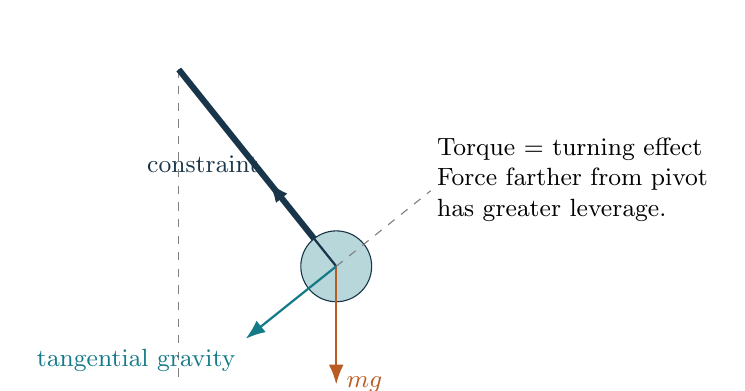
\begin{tikzpicture}
\coordinate(P)at(0,0);\coordinate(B)at(2,-2.5);\draw[ghost](P)--(0,-4);\draw[rod](P)--(B);\node[mass]at(B){};\draw[arr,warm](B)--++(0,-1.5)node[right]{\(mg\)};\draw[arr,ink](B)--++(-.85,1.06)node[above left]{constraint};\draw[arr,teal](B)--++(-1.15,-.92)node[below left]{tangential gravity};\draw[ghost](B)--++(1.2,.96);\node[align=left]at(5,-1.4){Torque = turning effect\\Force farther from pivot\\has greater leverage.};
\end{tikzpicture}\caption{A force diagram for a single mass on a rigid link. Tension/constraint force is not a separate integrated state in this game.}
\end{figure}
\textbf{Torque} means the turning effect of a force about the pivot. For gravity, the torque is \(-mg\ell\sin\theta\). The resistance to angular acceleration is the moment of inertia \(m\ell^2\). Dividing gives
\begin{equation}\label{eq:single}\ddot\theta=-\frac{g}{\ell}\sin\theta.\end{equation}
Mass cancels in this one-link idealization. A positive displacement accelerates back toward zero. At the lowest point, gravity's tangential component is zero, but velocity may be largest, so the bob passes through rather than stopping.
\subsection{Energy explains release height}
Kinetic energy is energy of motion; gravitational potential energy is energy associated with height. Relative to the bottom position,
\[
 K=\tfrac12 m\ell^2\omega^2,\qquad U=mg\ell(1-\cos\theta).
\]
Without damping, a moving pivot, or gameplay events, \(K+U\) stays constant in the exact mathematical model. Potential energy becomes kinetic energy during descent, then becomes potential energy again during ascent.

For release from rest at \(\theta_0\), energy conservation gives bottom speed
\[
 v_{\rm bottom}=\sqrt{2g\ell(1-\cos\theta_0)}.
\]
For \(\ell=2.5\), \(g=9.8\), and \(\theta_0=60^\circ\), this is approximately \(4.95\) model m/s. This calculation is a teaching example for one link, not an exact prediction for the game's two-link launch.
\begin{arcade}Energy is not generally conserved in a stage. Pulses, boosters and moving anchors can add energy. Damping and several collision rules remove it. Portals deliberately rewrite the state.\end{arcade}

\section{Small swings, large swings and damping}
For small angles measured in radians, \(\sin\theta\approx\theta\). Equation~\eqref{eq:single} then predicts a nearly sinusoidal swing with period
\[
 T_0=2\pi\sqrt{\ell/g}.
\]
The period is the time for a full back-and-forth cycle. For \(\ell=2.5\) and \(g=9.8\), \(T_0\approx3.17\) s. Large swings do not obey the small-angle approximation: their period becomes longer, and near an upward unstable position the timing becomes especially sensitive.
\begin{figure}[H]\centering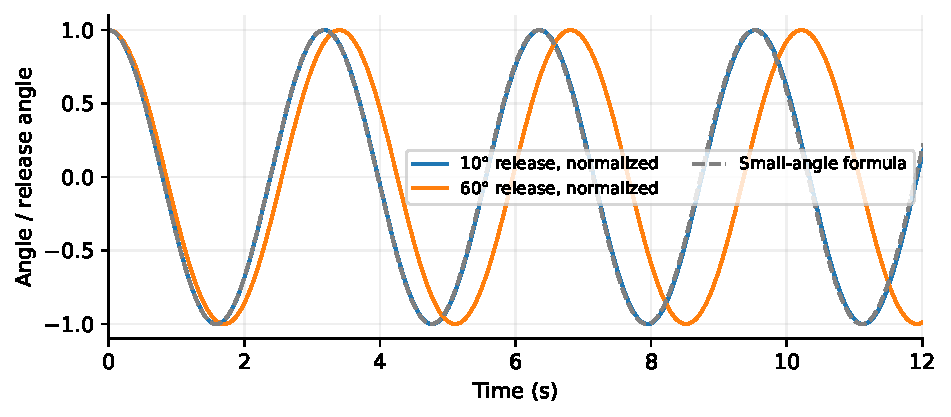
\includegraphics[width=\linewidth]{figures/oscillation.pdf}
\caption{Numerical one-link experiments using the game's \code{rk4} solver, with damping set to zero. Angles are normalized by their own release angles so timing differences are visible. The 60-degree trajectory lags the small-angle formula.}
\end{figure}
The actual solver adds velocity-proportional angular drag. For a single link at a fixed pivot and with no wind,
\[
 \ddot\theta=-\frac{g}{\ell}\sin\theta-c\dot\theta,
 \qquad c=0.04\ \mathrm{s}^{-1}\text{ normally}.
\]
Drag opposes the sign of motion. Near the small-angle regime, the amplitude envelope decays approximately like \(e^{-ct/2}\). The energy loss is
\[
 \frac{\dd E}{\dd t}=-cm\ell^2\omega^2\leq0.
\]
This sign check is useful: damping alone should not increase mechanical energy. For a multi-link chain, the damping is applied as a particular set of generalized torques, explained next; one cannot simply assume every angular acceleration independently receives \(-c\omega_i\).

\section{Two or more links: why they influence each other}
Moving link 1 moves every mass below it. Moving the last link affects only its own final mass directly. Consequently, the angular accelerations are coupled: the solver must find them together.
\begin{figure}[H]\centering
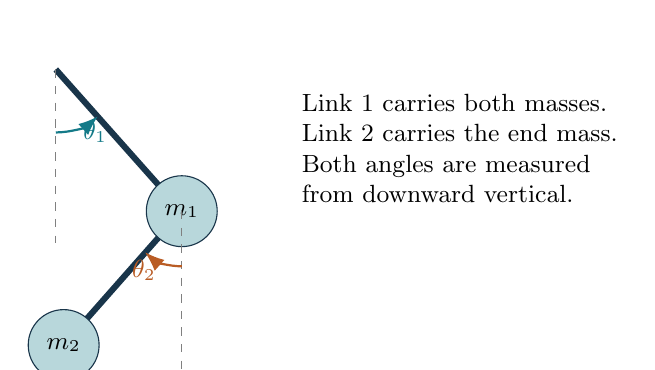
\begin{tikzpicture}
\coordinate(P)at(0,0);\coordinate(A)at(1.6,-1.8);\coordinate(B)at(.1,-3.5);\draw[rod](P)--(A)--(B);\node[mass]at(A){\(m_1\)};\node[mass]at(B){\(m_2\)};\draw[ghost](P)--(0,-2.2);\draw[ghost](A)--++(0,-2);\draw[arr,teal](0,-.8)arc(-90:-48:.8);\node[teal]at(.5,-.8){\(\theta_1\)};\draw[arr,warm](1.6,-2.5)arc(-90:-132:.7);\node[warm]at(1.12,-2.55){\(\theta_2\)};\node[align=left,anchor=west]at(3,-1){Link 1 carries both masses.\\Link 2 carries the end mass.\\Both angles are measured\\from downward vertical.};
\end{tikzpicture}\caption{Absolute angles and downstream loading in a two-link pendulum.}
\end{figure}
\subsection{A matrix is a compact set of simultaneous equations}
For two unknown accelerations, the equations have the form
\[
 M_{11}\alpha_1+M_{12}\alpha_2=B_1,\qquad
 M_{21}\alpha_1+M_{22}\alpha_2=B_2.
\]
The matrix \(M\) collects the coefficients and the vector \(B\) collects the driving terms:
\[
 \underbrace{\begin{pmatrix}M_{11}&M_{12}\\M_{21}&M_{22}\end{pmatrix}}_{\text{mass matrix}}
 \underbrace{\begin{pmatrix}\alpha_1\\\alpha_2\end{pmatrix}}_{\text{unknown accelerations}}
 =\underbrace{\begin{pmatrix}B_1\\B_2\end{pmatrix}}_{\text{gravity, coupling, forcing, drag}}.
\]
The mass matrix is not just a table of masses. It includes masses, link lengths and the current angles. The off-diagonal entries say that accelerating one angle is dynamically connected to accelerating another.
\subsection{The exact equations used by the code}
Number links and masses from \(1\) to \(N\), and define downstream mass
\[
 \mu_{ij}=\sum_{k=\max(i,j)}^N m_k.
\]
The matrix entries are
\begin{equation}\label{eq:M}M_{ij}=\mu_{ij}\ell_i\ell_j\cos(\theta_i-\theta_j).\end{equation}
At each derivative evaluation, the code solves \(M\vect\alpha=\vect B\), with
\begin{align}\label{eq:B}
 B_i={}&-\sum_{j=1}^N\mu_{ij}\ell_i\ell_j\sin(\theta_i-\theta_j)\omega_j^2\nonumber\\
 &-\mu_{ii}(g-a_y)\ell_i\sin\theta_i
 -\mu_{ii}(a_x-a_w)\ell_i\cos\theta_i
 -c\mu_{ii}\ell_i^2\omega_i.
\end{align}
Here \(a_x,a_y\) are the pivot's horizontal and downward accelerations, and \(a_w\) is the wind's horizontal acceleration. All accelerations in this formula are in model units, not pixels per second squared.

Read the four contributions in order:
\begin{enumerate}
\item \textbf{Velocity coupling:} other links' angular velocities affect this link's acceleration through the changing geometry.
\item \textbf{Effective gravity:} gravity is measured relative to the accelerating anchor.
\item \textbf{Horizontal forcing:} pivot acceleration and wind contribute with opposite signs.
\item \textbf{Damping torque:} this is proportional to \(\mu_{ii}\ell_i^2\omega_i\).
\end{enumerate}
The angles change \(M\) and \(B\), so the answer must be recomputed continuously. There is no single fixed table of accelerations for a stage.
\subsection{A worked two-link calculation}
With \(\ell_1=\ell_2=1.25\), \(m_1=m_2=1\), \(\theta_1=30^\circ\), \(\theta_2=-20^\circ\), zero starting velocity, a fixed anchor and no damping,
\[
 M\approx\begin{pmatrix}3.125&1.0044\\1.0044&1.5625\end{pmatrix},\quad
 B\approx\begin{pmatrix}-12.2500\\4.1897\end{pmatrix}.
\]
Solving gives \(\alpha_1\approx-6.0269\) and \(\alpha_2\approx6.5554\) rad/s\(^2\). The second acceleration is not just \(-g\sin\theta_2/\ell_2\): the moving first link changes the answer.

\section{Where the coupled equations come from}
This section is optional on a first reading. It explains why the matrix in equation~\eqref{eq:M} has its particular form.
\subsection{Write the energies}
Differentiate equation~\eqref{eq:positionN} for a fixed pivot:
\[
 \dot x_k=\sum_{i\leq k}\ell_i\cos\theta_i\,\omega_i,\qquad
 \dot y_k=-\sum_{i\leq k}\ell_i\sin\theta_i\,\omega_i.
\]
Adding each mass's kinetic energy gives
\begin{equation}\label{eq:T}
 T=\frac12\sum_k m_k(\dot x_k^2+\dot y_k^2)
 =\frac12\sum_{i,j}\mu_{ij}\ell_i\ell_j\cos(\theta_i-\theta_j)\omega_i\omega_j.
\end{equation}
Because downward \(y\) increases when gravitational potential falls,
\[
 U=-\sum_k m_kg y_k=-g\sum_i\mu_{ii}\ell_i\cos\theta_i+\text{constant}.
\]
\subsection{Use a compact mechanics rule}
Define the \emph{Lagrangian} \(\mathcal L=T-U\). This is a useful bookkeeping function, not a new force. The Euler--Lagrange equation for angle \(i\) is
\[
 \frac{\dd}{\dd t}\left(\frac{\partial\mathcal L}{\partial\omega_i}\right)
 -\frac{\partial\mathcal L}{\partial\theta_i}=Q_i.
\]
A partial derivative asks how a quantity changes when one input varies while the other inputs are temporarily held fixed. \(Q_i\) represents any extra generalized torque.

Differentiating the energies, collecting the terms containing \(\alpha_j\), and simplifying the angular-velocity terms gives
\[
 \sum_j M_{ij}\alpha_j+
 \sum_j\mu_{ij}\ell_i\ell_j\sin(\theta_i-\theta_j)\omega_j^2
 +\mu_{ii}g\ell_i\sin\theta_i=Q_i.
\]
The wind, anchor acceleration and damping torques supply the remaining parts of equation~\eqref{eq:B}. Ideal constraint forces do not have to be solved as separate unknowns because the angular coordinates already enforce link lengths.
\begin{idea}{Why this is better than guessing each link's motion}
Solving every link as if it were an independent pendulum would omit the off-diagonal mass terms and velocity coupling. It could draw a chain, but it would not reproduce the game's whip-like multi-link dynamics.
\end{idea}

\section{Launch settings, clones and sensitivity}
\subsection{What the starting sliders actually set}
For a stage with \(N\) links, the initial state is the array
\[
 \vect z=(\theta_1,\ldots,\theta_N,\omega_1,\ldots,\omega_N).
\]
The launch angle is assigned to \emph{every} link. The initial angular velocity is also assigned to every link. Because the angles are absolute, equal starting angles create a straight chain. This is different from setting the velocity of only the final bob.

For the standard chain, \(\ell_i=2.5/N\). A two-link chain has two links of length \(1.25\); a five-link chain has five of length \(0.5\). More links do not lengthen its maximum straight reach, but they add independent degrees of freedom. Because each point mass stays at 1, the total modeled mass also increases from 2 units for two links to 5 units for five links; the code does not keep total mass fixed when changing link count.
\subsection{Clones begin almost, but not exactly, together}
Clone \(c\), counting from zero, begins at angle
\[
 \theta_i(0)=\theta_{\rm launch}+0.001c.
\]
The offset is in radians: \(0.001\) rad is about \(0.0573^\circ\). It is intentionally tiny. The clones otherwise receive the same initial angular velocity and start a 3-second inter-clone collision cooldown so their overlapping launch does not immediately cause repeated collisions.
\subsection{Sensitivity is not randomness}
A nonlinear multi-link pendulum can amplify small initial differences. This is often described as chaotic behavior. A precise deterministic equation can be difficult to predict far into the future without being random.
\begin{figure}[H]\centering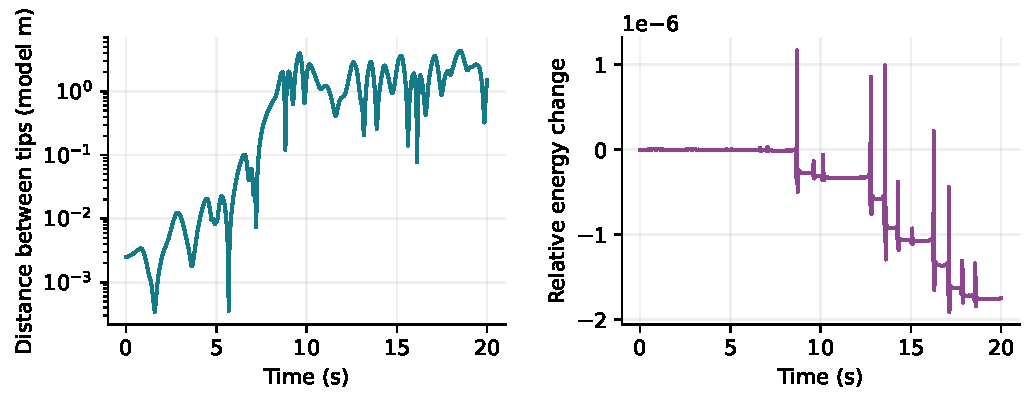
\includegraphics[width=\linewidth]{figures/sensitivity.pdf}
\caption{Two isolated two-link chains released at 120 degrees, differing by 0.001 rad in each angle. Left: their tip separation. Right: relative energy error for one chain with no damping. Data come from the game's solver at a step of 1/240 s, without stage collisions. Growth of separation illustrates sensitivity; this plot alone is not a formal proof of chaos or a measured Lyapunov exponent.}
\end{figure}
The game also has discontinuous events: a tiny change can make a bob hit a bomb rather than miss it. Those events can magnify differences much more abruptly than free pendulum motion. Random spark directions are visual effects, not the source of the basic pendulum equations.

\section{How the computer advances time}
\subsection{A simulation uses small steps}
A browser cannot solve the complete future trajectory in one exact calculation. It stores the current state and advances by a short interval \(h\). The derivative function returns
\[
 f(\vect z,t)=(\omega_1,\ldots,\omega_N,\alpha_1,\ldots,\alpha_N).
\]
Even the elementary approximation \(\vect z_{n+1}\approx\vect z_n+h f(\vect z_n)\) has meaning: take the current rate of change and apply it briefly. But that simple Euler step can distort pendulum energy noticeably.
\subsection{The fourth-order Runge--Kutta method (RK4)}
The game samples four tentative rates before taking one step:
\begin{align*}
 k_1&=f(z_n),& k_2&=f(z_n+hk_1/2),\\
 k_3&=f(z_n+hk_2/2),&k_4&=f(z_n+hk_3),\\
 z_{n+1}&=z_n+\frac h6(k_1+2k_2+2k_3+k_4).
\end{align*}
Each \(k\) is a vector, so all angles and velocities are updated together. Each evaluation constructs and solves the mass matrix. The implementation passes the current forcing values into those evaluations; wind and anchor acceleration are not independently resampled at each RK4 midpoint.
\begin{figure}[H]\centering
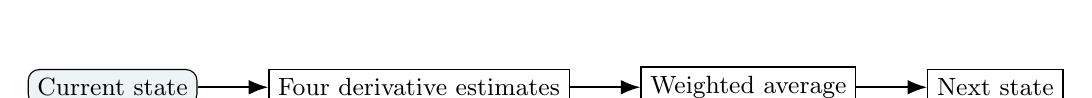
\begin{tikzpicture}[node distance=9mm]
\node[draw,rounded corners,fill=teal!8] (s){Current state};\node[draw,right=of s](k){Four derivative estimates};\node[draw,right=of k](w){Weighted average};\node[draw,right=of w](n){Next state};\draw[arr](s)--(k);\draw[arr](k)--(w);\draw[arr](w)--(n);
\end{tikzpicture}\caption{RK4 takes several tentative looks ahead. These temporary states are not extra visible bobs and do not represent simultaneously existing objects.}
\end{figure}
\subsection{Solving the matrix}
\code{solveMatrix} uses Gaussian elimination with row swaps chosen from the largest available pivot magnitude (partial pivoting). It eliminates unknowns from successive rows, then works backward to recover the accelerations. Divisions by very small numbers are skipped at a threshold of \(10^{-12}\). That is a numerical safeguard, not a physical model of a degenerate chain.
\subsection{Frames and substeps are different}
Normal gameplay clamps a browser-frame interval to at most \(0.03\) s. It then divides scaled time into four integration substeps. At 60 frames/s and ordinary time scale,
\[
 \Delta t\approx1/60,\qquad h=\Delta t/4\approx1/240\text{ s}.
\]
At 120 frames/s, those integration substeps are smaller. Many gameplay contacts are checked only in the \emph{last} substep of each frame, while inter-bob checks occur after each substep. This difference matters for repeatability and fast motion.

\section{Gravity: normal, low, heavy, inverted and zero}
The standard solver gravity is \(g=9.8\) in model m/s\(^2\), positive downward. Low and heavy gravity stages choose different values. A smaller positive \(g\) generally makes the swing slower; a larger \(g\) makes it faster. For a one-link small swing, frequency scales like \(\sqrt{g/\ell}\), not directly like \(g\).
\begin{figure}[H]\centering
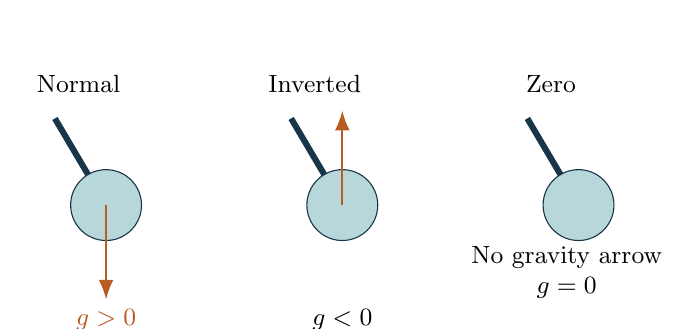
\begin{tikzpicture}
\foreach \x/\lab/\dir in {0/Normal/-1,3/Inverted/1,6/Zero/0}{\draw[rod](\x,0)--++(.65,-1.1);\node[mass]at(\x+.65,-1.1){};\node[above]at(\x+.3,.2){\lab};}
\draw[arr,warm](.65,-1.1)--(.65,-2.3)node[below]{\(g>0\)};\draw[arr,warm](3.65,-1.1)--(3.65,.1);\node[below]at(3.65,-2.3){\(g<0\)};\node[below,align=center]at(6.5,-1.5){No gravity arrow\\\(g=0\)};
\end{tikzpicture}\caption{Changing the sign or magnitude of gravity changes the restoring tendency. Zero gravity does not remove rod constraints or damping.}
\end{figure}
In inverted gravity, upward becomes the preferred direction. Periodic inversion stages multiply the current gravity by \(-1\) when a stage-specific countdown expires. This flips the acceleration field; it does not instantly reverse the current velocities. Motion continues through the transition.

In Zero Gravity, \(g=0\). A motionless chain at a fixed pivot with no other forces remains motionless. If it already moves, inertial coupling and constraints still affect its path, and damping still removes energy. ``Zero gravity'' is not ``all forces turned off.''

\section{Moving pivots and rails}
\subsection{An accelerating support changes the apparent force}
Imagine standing in a vehicle that accelerates right: relative to the vehicle, you seem pushed left. A pendulum on a moving support behaves similarly. The solver uses effective acceleration
\[
 \vect g_{\rm effective}=(a_w-a_x,\ g-a_y).
\]
The pivot's \emph{acceleration}, not simply its position, drives these additional terms. Moving anchors can exchange energy with a pendulum because the support is externally prescribed, like a motorized apparatus.
\begin{figure}[H]\centering
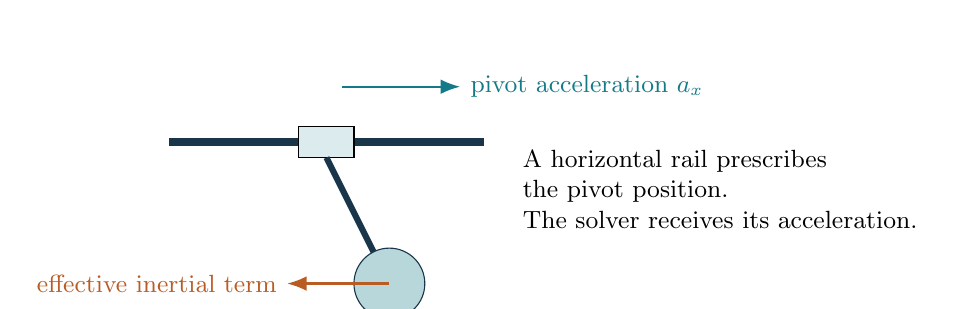
\begin{tikzpicture}
\draw[ink,line width=3pt](-2,0)--(2,0);\draw[fill=teal!15](-.35,-.2)rectangle(.35,.2);\draw[rod](0,-.2)--(.8,-1.8);\node[mass]at(.8,-1.8){};\draw[arr,teal](.2,.7)--(1.7,.7)node[right]{pivot acceleration \(a_x\)};\draw[arr,warm](.8,-1.8)--(-.5,-1.8)node[left]{effective inertial term};\node[align=left]at(5,-.6){A horizontal rail prescribes\\the pivot position.\\The solver receives its acceleration.};
\end{tikzpicture}\caption{The reference frame attached to the pivot is accelerating.}
\end{figure}
\subsection{The prescribed rail motion}
For horizontal amplitude \(A_x\) in pixels,
\[
 x_p=x_0+A_x\sin(\Omega_x t+\phi_x),\qquad
 a_x=-\frac{A_x}{s}\Omega_x^2\sin(\Omega_x t+\phi_x).
\]
The vertical equation is analogous, using \(A_y,\Omega_y,\phi_y\). Here \(\Omega\) is a prescribed rail frequency in rad/s, not a bob's angular velocity. Doubling frequency multiplies acceleration amplitude by four.

Equal frequencies with a quarter-cycle phase offset can create an elliptical orbit; equal amplitudes give a circle. Different frequencies can produce more complicated two-axis paths. The two coordinates are computed independently. In the release, visible horizontal/vertical rail tracks follow the carriage's current coordinates rather than assuming every two-axis path is an ellipse.

The rail also acts as a gameplay obstacle. Its contact geometry and bounce rule are described in Section~\ref{sec:contacts}; motorized support motion and rail collision are separate mechanisms.

\section{Wind: a horizontal acceleration, not a fluid simulation}
A constant wind is stored as a horizontal acceleration input. A gusting wind uses
\[
 a_w(t)=f+A\sin(\Omega t+\phi).
\]
The baseline \(f\) biases one direction, amplitude \(A\) controls the variation, and \(\phi\) sets the initial phase. The direction reverses only if the complete expression crosses zero; a gust need not reverse just because it varies.
\begin{figure}[H]\centering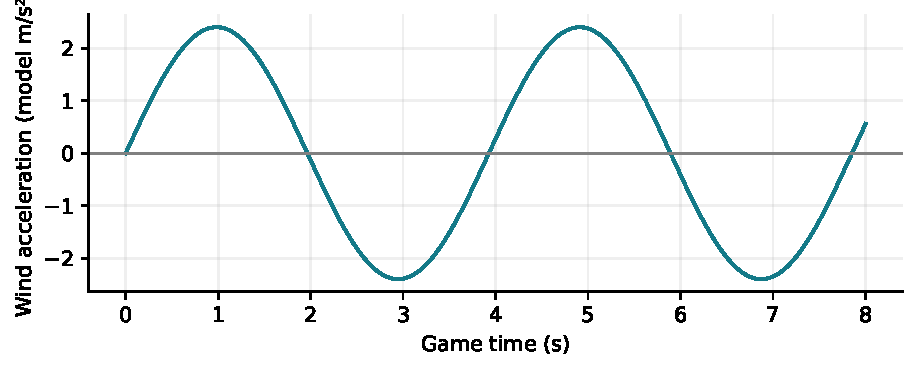
\includegraphics[width=\linewidth]{figures/wind.pdf}
\caption{Example authored gust parameters: \(f=0\), \(A=2.4\), \(\Omega=1.6\), \(\phi=0\). Positive acceleration pushes right; negative pushes left. This is an illustrative input curve, not a universal stage setting.}
\end{figure}
For a single link, combining wind, moving support and damping gives
\[
 \ddot\theta=-\frac{g-a_y}{\ell}\sin\theta
 +\frac{a_w-a_x}{\ell}\cos\theta-c\dot\theta.
\]
This compact equation is a useful bridge between the basic pendulum and the full mass-matrix model.
\begin{arcade}Although the HUD labels wind in m/s, the value is used by the equations as an \emph{acceleration}. The game does not solve air velocity, pressure, turbulence, or speed-dependent aerodynamic drag. This is an interface-unit mismatch in the release, not a reason to reinterpret the implemented formula.\end{arcade}
Wind artwork is separate from wind dynamics. Its scrolling offset is based on an integral of the authored wind curve, scaled by 32 for visual motion. Reduced-motion settings may hold this artwork still; the acceleration field remains unchanged.

\section{Pulses and boost rings add angular velocity}
\subsection{A pulse is an instantaneous state change}
During play, a pulse affects each living chain's \emph{last} angular velocity:
\[
 \omega_N\leftarrow\begin{cases}\omega_N+2.5,&\omega_N\geq0,\\\omega_N-2.5,&\omega_N<0.\end{cases}
\]
It reinforces the current rotation direction; at exactly zero it chooses the positive direction. The player does not aim an arbitrary spatial force by tapping a point. A pulse consumes one available charge and creates sound and visual effects.
\begin{figure}[H]\centering
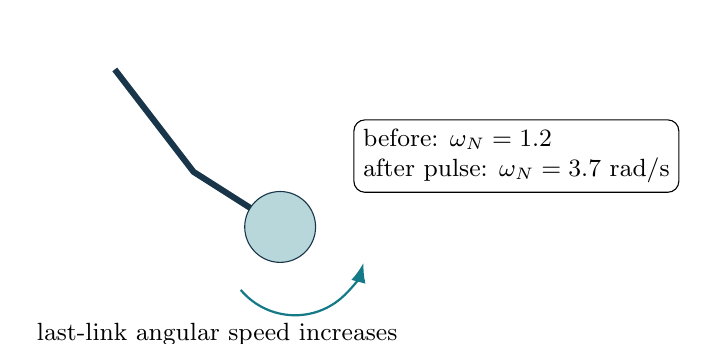
\begin{tikzpicture}
\draw[rod](0,0)--(1,-1.3)--(2.1,-2);\node[mass]at(2.1,-2){};\draw[arr,teal](1.6,-2.8)arc(-140:-15:.9);\node[below]at(1.3,-3.1){last-link angular speed increases};\node[draw,rounded corners,align=left]at(5.1,-1.1){before: \(\omega_N=1.2\)\\after pulse: \(\omega_N=3.7\) rad/s};
\end{tikzpicture}\caption{A pulse adds angular velocity to the tip link, after which the coupled solver redistributes motion through the chain.}
\end{figure}
\subsection{Boost rings use a similar rule}
A ring triggers when the tip's collision circle overlaps it. The game adds the ring's \code{boostSpd} to \(\omega_N\), with the sign of the current rotation (positive if zero). A \(0.4\)-s cooldown reduces repeated activation.

The displayed chevron angle is artwork; the implemented impulse is not a Cartesian launch along that arrow. It is an angular-velocity increment. With several links, the eventual tip direction depends on all link angles and velocities.
\begin{arcade}Neither a pulse nor a boost is computed from a physical impulse and an effective mass. These are arcade controls intended to boost motion, applied on top of the mechanically coupled motion.\end{arcade}
For one link, a change \(\Delta\omega\) changes kinetic energy by
\[
 \Delta K=\tfrac12m\ell^2\big[(\omega+\Delta\omega)^2-\omega^2\big].
\]
For a multi-link chain, off-diagonal kinetic-energy terms also matter. Increasing the last-link speed does not, by itself, mathematically guarantee an increase in total chain kinetic energy; cross terms depend on the other links.

\section{Detecting contact}\label{sec:contacts}
\subsection{Two circular hit areas}
For tip center \(P=(x,y)\), object center \(C\), and radii \(r_b,r_o\), the usual test is
\[
 d=\sqrt{(x-C_x)^2+(y-C_y)^2}<r_b+r_o.
\]
It tests overlap, not only whether the center enters the target.
\begin{figure}[H]\centering
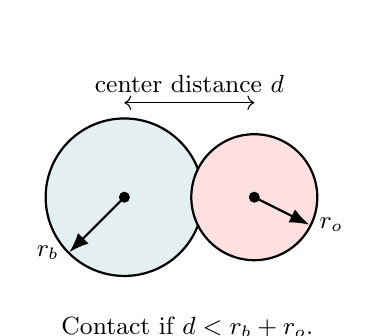
\begin{tikzpicture}
\draw[fill=teal!12,thick](0,0)circle(1);\fill(0,0)circle(2pt);\draw[fill=red!12,thick](1.65,0)circle(.8);\fill(1.65,0)circle(2pt);\draw[<->](0,1.2)--(1.65,1.2)node[midway,above]{center distance \(d\)};\draw[arr](0,0)--(-.7,-.7)node[left]{\(r_b\)};\draw[arr](1.65,0)--(2.35,-.35)node[right]{\(r_o\)};\node[below]at(.8,-1.4){Contact if \(d<r_b+r_o\).};
\end{tikzpicture}\caption{Collision geometry uses the sum of the radii. Glow, sparks and trails do not enlarge the physical hit area.}
\end{figure}
Standard bob radius starts at 21 pixels. Destroying a directly contacted target grows it by 4.5 pixels, up to 54. Certain hazards shrink an enlarged bob by 4.5 pixels, never below 21. The temporary \code{popScale} squash/stretch is visual and is not included in the circle-contact radius.

Many authored circular objects and force-field cores are scaled by 1.5 for readability and matching contact sizes. Positions, stage link lengths, rectangular zones and force influence radii are not all scaled together. A static gap for the largest bob needs at least \(2\times54=108\) pixels of free clearance, plus any desired margin.
\subsection{A circle near a laser or gate segment}
For segment endpoints \(A,B\), first project \(P\) onto the infinite line, then clamp to the segment:
\[
 u=\operatorname{clamp}\!\left(\frac{(P-A)\cdot(B-A)}{\lVert B-A\rVert^2},0,1\right),\qquad C=A+u(B-A).
\]
Test \(\lVert P-C\rVert<r_b+r_s\), where the implemented half-thickness \(r_s=3\) pixels. The denominator is guarded for a zero-length segment.
\begin{figure}[H]\centering
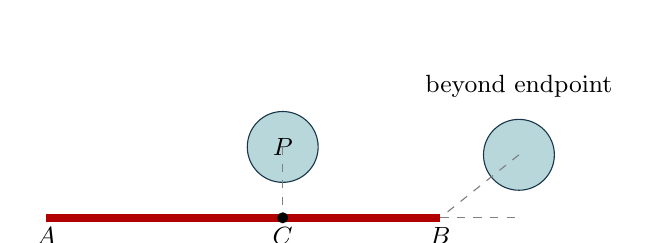
\begin{tikzpicture}
\draw[line width=3pt,red!70!black](0,0)--(5,0);\node[below]at(0,0){\(A\)};\node[below]at(5,0){\(B\)};\node[mass]at(3,.9){\(P\)};\draw[ghost](3,.9)--(3,0);\fill(3,0)circle(2pt);\node[below]at(3,0){\(C\)};\draw[ghost](5,0)--(6,0);\node[mass]at(6,.8){};\draw[ghost](6,.8)--(5,0);\node[above]at(6,1.4){beyond endpoint};
\end{tikzpicture}\caption{Closest-point distance handles contacts near the middle and at either endpoint.}
\end{figure}
\subsection{Which part of the chain can touch what?}
\begin{center}\begin{tabular}{p{.41\linewidth}p{.49\linewidth}}
\toprule Object/test & Tested part of a living chain\\\midrule
Target, bomb, bumper, portal, ring & Tip circle\\
Laser, closed gate & Tip circle against line segment\\
Slime/resin & Tip center inside rectangle\\
Rail & Joint positions, including the tip, with different radii\\
Force-field influence & Each joint position\\
Black-hole death & Tip overlapping core\\
Another clone & Tip circle against tip circle\\\bottomrule
\end{tabular}\end{center}
A rod can visually cross a laser without its tip crossing the laser. That alone does not satisfy the implemented tip-contact test. Likewise, there is no universal solid wall at every canvas edge: the release handles authored obstacles and rails, not a general bouncing border. Decorative boundaries and rod thickness should not be mistaken for extra collision geometry.

\subsection{A frame can miss a fast crossing}
Most target, portal, bumper and segment tests use the computed end-of-frame tip position, not a swept path between its old and new positions. A very fast bob can cross a thin obstacle without an end sample inside it. Four integration substeps improve motion integration but do not turn those contact tests into continuous collision detection.

\section{Bumpers, springs, absorbers, rails and clones}
\subsection{What a physically complete bounce would do}
For a free ball at a fixed wall, let \(\vect n\) be the outward unit normal and \(e\) a coefficient of restitution. A common idealized response is
\[
 \vect v'=\vect v-(1+e)(\vect v\cdot\vect n)\vect n.
\]
It reverses and scales only the normal component, while leaving tangential velocity unchanged. Applying an impulse to a constrained multi-link chain would require mapping it through the chain's geometry and mass matrix.
\subsection{What the release actually does}
The game's normal bumper response is much simpler:
\[
 \omega_N\leftarrow q\omega_N.
\]
Typical normal bumpers use \(q=-0.8\), springs use values less than \(-1\), and absorbers use a small magnitude such as \(-0.05\). The minus sign reverses the last link's rotation. Spring multipliers larger than one in magnitude inject motion; absorbers strongly reduce that component.

The stored property is named \code{restitution}, but it is a signed angular-velocity multiplier, not the standard normal restitution coefficient \(e\). Multiplying only \(\omega_N\) does not guarantee a particular whole-chain energy change. Moving bumpers follow an authored sinusoidal horizontal path; their contact response does not explicitly add their own surface velocity to a momentum calculation.
\subsection{Rails and gates}
Closed gates reverse and scale the final angular velocity by \(-0.8\) and trigger shrinking. Rail contacts can involve intermediate joints as well as the tip; a rail hit multiplies \emph{all} angular velocities by \(-0.8\), with a 0.08-s cooldown. Rail contact half-width is 18 pixels, and intermediate-joint radius is 7.5 pixels. A vertical-track test also excludes contacts very near the pivot.

The rail geometry consists of axis-aligned tracks through the current pivot with extents based on the authored amplitudes and extra 30-pixel end margins. These are not collision tests against a thick ellipse, even when the pivot's prescribed path is elliptical.
\subsection{Clone--clone contacts}
Overlapping living tips with expired cooldowns use
\[
 \omega'_A=-0.85\omega_A+0.3\omega_B,\qquad
 \omega'_B=-0.85\omega_B+0.3\omega_A.
\]
Here \(\omega_A,\omega_B\) are the old last-link angular velocities. A 0.06-s cooldown prevents immediate repeated activation.
\begin{arcade}The clone routine computes geometric normal and tangent directions, but those values are not used in its final velocity update. Despite a source comment referring to elastic exchange, this rule is not a full conservation-of-momentum impulse solver. There is also no general overlap-position correction.\end{arcade}

\section{Targets, armor, bombs, switches and lasers}
\subsection{Targets and armor}
A normal target disappears on circular overlap. It does not produce a physically calculated reaction impulse. Direct destruction grows the bob. An armored non-bomb target with more than one hit point loses one hit point and applies \(\omega_N\leftarrow-0.6\omega_N\). The last hit destroys it normally.

There is no general target-contact debounce equivalent to the ring cooldown. Consecutive sampled overlaps can therefore count as repeated armored hits. Descriptions such as ``two hits'' refer to the coded health events, not necessarily two visibly separated full swings.
\subsection{Bombs}
Directly contacting a bomb destroys it and triggers an explosion. Every living \emph{non-bomb} target whose center is within 145 pixels of the bomb center is cleared, including armored targets, and receives its explosion score. This uses target-center distance, not target-radius overlap with the blast.
\begin{figure}[H]\centering
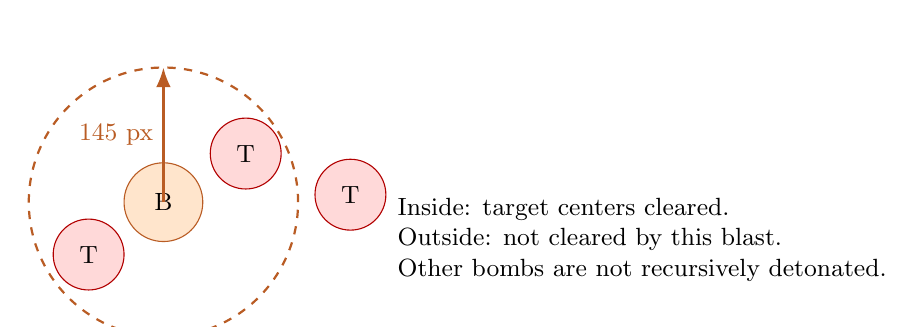
\begin{tikzpicture}[scale=.95]
\draw[dashed,warm,thick](0,0)circle(1.8);\node[circle,draw=warm,fill=orange!20,minimum size=10mm]at(0,0){B};\node[target]at(1.1,.65){T};\node[target]at(-1,-.7){T};\node[target]at(2.5,.1){T};\draw[arr,warm](0,0)--(0,1.8)node[midway,left]{145 px};\node[align=left,anchor=west]at(3,-.5){Inside: target centers cleared.\\Outside: not cleared by this blast.\\Other bombs are not recursively detonated.};
\end{tikzpicture}\caption{The bomb's clearance radius is a gameplay rule. Its shockwave picture is not a simulated pressure field.}
\end{figure}
The release's explosion function does \emph{not} recursively trigger other bombs, and it does not calculate an outward mechanical impulse on the pendulum. ``Chain explosion'' can describe clearing a group of targets, but it should not be read as a full bomb-to-bomb detonation model.
\subsection{Switches and timed gates}
Touching a switch activates its gate for an authored duration (default 4.5 s). The countdown then closes it again. The gate's open state is a discrete rule; no hinge, motor torque, or moving-door dynamics is integrated.
\subsection{Lasers and shields}
A laser segment hit consumes a shared shield life, shrinks the bob if possible, and multiplies all of that chain's angular velocities by \(-0.85\). A shared 0.55-s laser cooldown limits repeated hits. On the last life, that chain is marked dead; failure occurs when all chains are dead while playing.

A glowing emitter, fuse, spring tail, or force-field aura is not automatically part of a lethal hit shape. Contact is determined by the specific circle, segment or core test, not the extent of every visible effect.

\section{Black holes and repulsor fields}
These gimmicks alter angular velocities after the RK4 motion step. They are not Newtonian astrophysical gravity and do not model spacetime or general relativity.

For a joint at \(J\) and field center \(C\), define \(d=\lVert J-C\rVert\), outward unit vector \(\vect u=(J-C)/d\), and link tangent
\[
 \vect t_k=(\cos\theta_k,-\sin\theta_k).
\]
A field's influence is tested for each joint, inside its pull radius \(R\), with a lower distance guard \(d>1\) pixel.
\begin{figure}[H]\centering
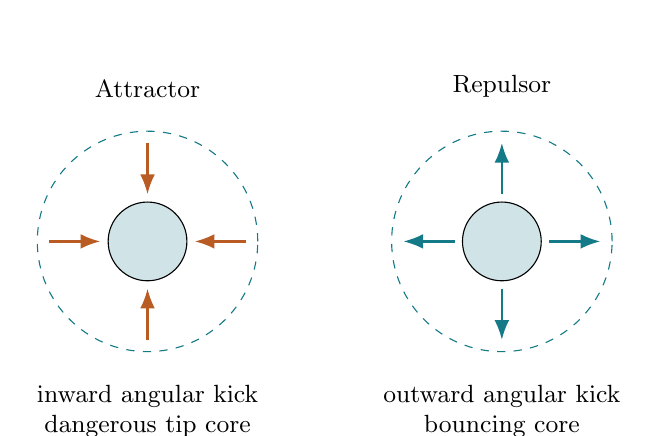
\begin{tikzpicture}
\foreach \x/\name in {0/Attractor,4.5/Repulsor}{\draw[dashed,teal](\x,0)circle(1.4);\node[circle,draw,fill=teal!20,minimum size=10mm]at(\x,0){};\node[above]at(\x,1.7){\name};}
\foreach \a in {0,90,180,270}{\draw[arr,warm]({1.25*cos(\a)},{1.25*sin(\a)})--({.6*cos(\a)},{.6*sin(\a)});\draw[arr,teal]({4.5+.6*cos(\a)},{.6*sin(\a)})--({4.5+1.25*cos(\a)},{1.25*sin(\a)});}
\node[below,align=center]at(0,-1.7){inward angular kick\\dangerous tip core};\node[below,align=center]at(4.5,-1.7){outward angular kick\\bouncing core};
\end{tikzpicture}\caption{Influence region and core are distinct. The formulas below are the implemented arcade field rules.}
\end{figure}
\subsection{Attractor (black hole)}
Inside the influence radius, the code applies
\[
 \Delta\omega_k=0.15\left(-\vect u\cdot\vect t_k\right)
 \left(1-\frac dR\right)S\,h,
\]
where \(S\) is the authored \code{pullStrength} and \(h\) is the integration substep duration supplied to this event block. The falloff is linear with distance to the edge, not \(1/d^2\). It is a tangential angular kick, without a consistent force-to-torque mass/length conversion.

If the \emph{tip} overlaps the core (using core radius plus effective tip radius) before the stage is won, the chain dies. Intermediate joints receive the field kick but do not trigger the same black-hole death rule. A guard prevents a completed stage from being turned into a black-hole loss.
\subsection{Repulsor}
Let core radius be \(r_c\), and define
\[
 \rho=\max\left(0.08,\frac{d-r_c}{R-r_c}\right),\qquad
 A_r=\frac{1.8|S|}{\rho^2}.
\]
The angular kick is
\[
 \Delta\omega_k=0.07(\vect u\cdot\vect t_k)A_r h.
\]
The lower bound on \(\rho\) limits the otherwise rapidly increasing near-core expression. At core overlap, the joint angular velocity is multiplied by \(-0.85\), with a bounce effect instead of black-hole death.
\begin{arcade}These field blocks are evaluated in the last-substep event section, but their increments are weighted by \(h=\Delta t/4\). They are not integrated as additional continuous forces inside every RK4 derivative evaluation. Treat the constants as tuned gameplay strengths, not universal physical constants.\end{arcade}

\section{Portals: rebuilding a chain near an exit}
A portal does more than translate a bob. The chain must still satisfy fixed link lengths after the jump. The code therefore rewrites its angles and angular velocities.
\subsection{Entry and reach limits}
An entrance is a portal with a destination ID. It activates when the tip distance is less than
\[
 1.55\times0.85\,r_{\rm portal}+r_b.
\]
A 0.65-s cooldown limits immediate repeat activation. Let exit displacement from the current pivot be \((d_x,d_y)\). The desired direction is \(\alpha=\operatorname{atan2}(d_x,d_y)\), consistent with angles measured from downward vertical. Desired distance is clamped to at most 98.5\% of the straight-chain reach.
\begin{figure}[H]\centering
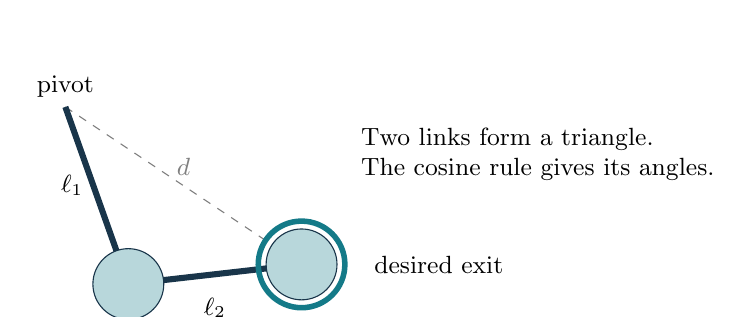
\begin{tikzpicture}
\coordinate(P)at(0,0);\coordinate(E)at(3,-2);\coordinate(J)at(.8,-2.25);\draw[ghost](P)--(E)node[midway,above]{\(d\)};\draw[rod](P)--(J)--(E);\node[mass]at(J){};\node[mass]at(E){};\draw[teal,line width=2pt](E)circle(.55);\node[above]at(P){pivot};\node[right=8mm]at(E){desired exit};\node[left]at(.35,-1){\(\ell_1\)};\node[below]at(1.9,-2.3){\(\ell_2\)};\node[align=left]at(6,-.6){Two links form a triangle.\\The cosine rule gives its angles.};
\end{tikzpicture}\caption{Two-link inverse kinematics: find angles that place a tip at a desired reachable point.}
\end{figure}
For two links, the implementation uses the cosine rule:
\[
 \beta=\arccos\frac{\ell_1^2+d^2-\ell_2^2}{2\ell_1d},\qquad
 \gamma=\arccos\frac{\ell_1^2+\ell_2^2-d^2}{2\ell_1\ell_2}.
\]
Here lengths and \(d\) must be in the same units (the code uses pixels). With a side choice \(b=\pm1\), it sets
\[
 \theta_1=\alpha+b\beta,\qquad\theta_2=\theta_1-b(\pi-\gamma).
\]
For more than two links, it instead fans the angles by 0.16 rad around \(\alpha\); it is not an exact general inverse-kinematics solve. Exits beyond maximum reach are approximated rather than reached exactly.
\subsection{Exit speed is a new assignment}
If the old last-link angular-speed magnitude is \(|\omega_N|\), define
\[
 w_e=\max(0.5,\,0.4|\omega_N|),\qquad
 \omega_k\leftarrow\sigma w_e\left(0.65+0.35\frac{k-1}{N-1}\right),
\]
with \(\sigma\) chosen from which side of the base pivot the exit lies. The denominator has a one-link safeguard in code. The trail is reset to the destination.
\begin{arcade}This does not preserve kinetic energy, linear momentum, or incoming direction. The visible ``0.6x'' warp message in the release differs from the implemented 0.4 angular-speed factor (with a 0.5 minimum). The equations above follow the code.\end{arcade}

\section{Slime, resin and timing effects}
\subsection{Zones damp angular motion}
A rectangular zone tests whether the tip center lies within its bounds. It does not use a circle--rectangle overlap with the tip radius. If it is inside, the game's code both increases the solver damping coefficient and explicitly applies
\[
 \omega_i\leftarrow\omega_i e^{-4Dh}
\]
for all links before an RK4 step. \(D\) is the zone's damping property (with code fallbacks). These are two damping mechanisms together, not just a material texture.

Only the first overlapping zone in the zone list is used on a substep; multiple overlapping zones are not added. The terms ``slime'' and ``resin'' select visual styling and authored damping values, not a fluid solver or a modeled adhesive constraint.
\subsection{Hit-stop, slow motion and pause}
Some hits set a short hit-stop timer. While it is positive, \code{update} reduces the timer and returns before advancing the ordinary physics. Stage-clear motion uses a time scale of 0.2; the result overlay appears after the separate clear countdown.

PAUSE suspends the game animation and associated game timers until explicit RESUME. A wall-clock second, a simulated game second, and a verification playback second are therefore not always interchangeable. The regular frame cap also means a long browser stall does not cause the physics to catch up by simulating all lost time in one large step.
\subsection{Why timing changes outcomes}
With only smooth ideal dynamics, smaller steps reduce integration error. Once a stage has sampled contacts, velocity kicks, cooldowns and state transitions, a slight timing shift can move a contact to a different side of a threshold. That can change a whole run, especially in a multi-link chain. Exact agreement across refresh rates is not established merely by using RK4.

\section{One frame in the release: an implementation map}
The simplified execution order below explains which mechanisms belong to the continuous pendulum model and which are event rules. It intentionally omits purely decorative bookkeeping.
\begin{figure}[H]\centering
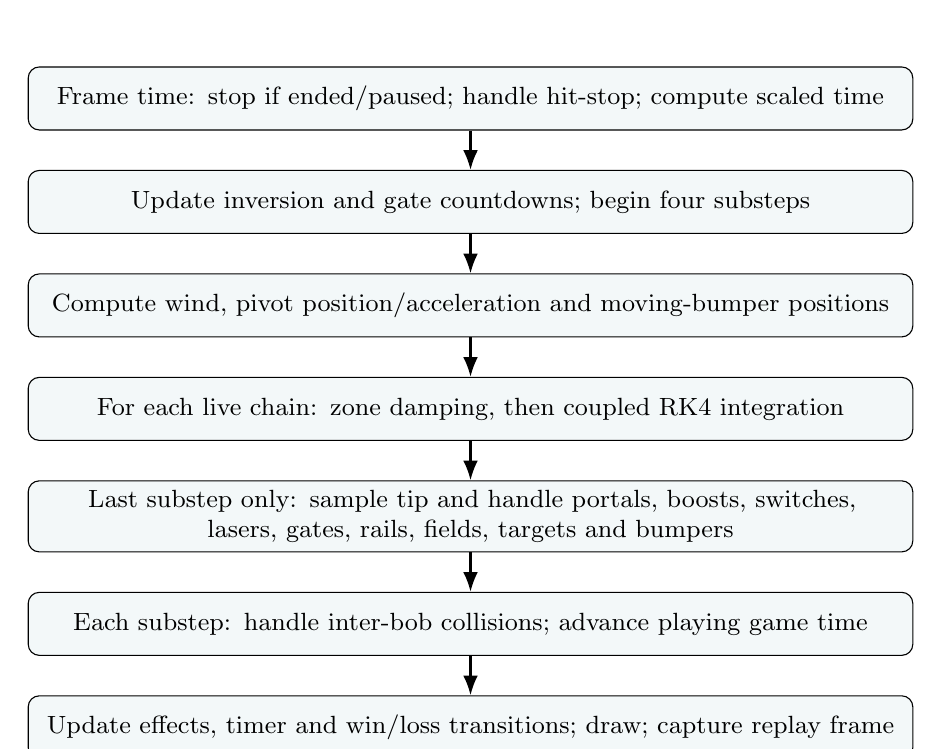
\begin{tikzpicture}[node distance=5mm,every node/.style={font=\small,align=center},box/.style={draw,rounded corners,text width=11cm,minimum height=8mm,fill=teal!5}]
\node[box](a){Frame time: stop if ended/paused; handle hit-stop; compute scaled time};
\node[box,below=of a](b){Update inversion and gate countdowns; begin four substeps};
\node[box,below=of b](c){Compute wind, pivot position/acceleration and moving-bumper positions};
\node[box,below=of c](d){For each live chain: zone damping, then coupled RK4 integration};
\node[box,below=of d](e){Last substep only: sample tip and handle portals, boosts, switches,\\lasers, gates, rails, fields, targets and bumpers};
\node[box,below=of e](f){Each substep: handle inter-bob collisions; advance playing game time};
\node[box,below=of f](g){Update effects, timer and win/loss transitions; draw; capture replay frame};
\foreach \u/\v in {a/b,b/c,c/d,d/e,e/f,f/g}{\draw[arr](\u)--(\v);}
\end{tikzpicture}\caption{High-level update order. The actual source is the final reference for detailed branch conditions.}
\end{figure}
The last-substep event block initially computes one tip position. Some events then change the chain state, but subsequent checks in that same block can still use the earlier sampled position until the next integration pass. This is another reason not to regard the event system as a simultaneous, exact contact solver.

Cooldowns serve a different purpose from integration substeps: they suppress particular repeated events. Not every contact type has a cooldown, and some cooldown updates are themselves tied to particular event-block frequencies.

\section{What is visual, what changes physics, and what affects score}
\begin{longtable}{p{.27\linewidth}p{.63\linewidth}}
\toprule\textbf{Feature}&\textbf{Role in the release}\\\midrule\endhead
Rod/link lengths&Constrain positions and enter the mass matrix.\\
Stored angular velocities&Determine future motion; changed by forces and event rules.\\
Bob collision radius&Changes contact thresholds; does not change modeled mass.\\
Glow, orbit-style trails, sparks&Artwork/history. They are not additional masses, force sources, or future positions.\\
Squash/stretch scale&Visual animation, distinct from collision radius.\\
Wind arrows&Visualize the authored field; do not themselves push the chain.\\
Prediction trail&A simplified preview, not a guaranteed future trajectory.\\
Recorded last attempt&Images from a prior run; viewing them does not rerun the physics.\\
Verification viewer&Re-simulates saved inputs at a fixed frame interval; different from image replay.\\
Score and stars&Rewards based on game events/time/pulses, not physical energy.\\\bottomrule
\end{longtable}
\subsection{Prediction is deliberately incomplete}
The aiming preview advances a copied chain for 50 steps of 0.02 s. It uses simplified inputs and does not reproduce all collisions, fields, portals, changing wind or gameplay state. Its anchor phase handling is also simpler than the live update. Treat it as an aiming aid, not a mathematical promise that the tip will follow the exact drawn line.
\subsection{Rewards are not conservation laws}
Ordinary target scoring uses a combo counter: \(100+50(\mathrm{combo}-1)\), with a 1.25-s combo window. Explosion-cleared targets receive their own 100-point award. Clear score adds a rounded time bonus of 100 times remaining game seconds (for finite timed stages).

A clear earns one star; another comes from leaving at least one pulse (automatic when pulses are locked), and another from retaining at least 35\% of the time limit. None of these numbers is kinetic energy or a physical efficiency measure.

\section{Reading the 250-stage verification correctly}
The release includes successful saved solutions for all 250 substages, independently replayed through the actual STAGE CLEAR result. The verification harness uses the same game update path with fixed outer-frame interval \(1/60\) s, four integration substeps, and pulse events on specified frame numbers. Player saves are isolated in memory.

This establishes a reproducible completion under that timing model. It does \emph{not} establish that every human input near the solution succeeds, that the solution is comfortable on mobile, that a gimmick must be used to win, or that variable frame timing produces a pixel-identical run.
\begin{idea}{Example: the user-guided Stage 44-2 solution}
Launch at \(-105^\circ\) and angular velocity \(-1.2\) rad/s. Apply automated pulses on frames 36 and 100: playback times 0.60 s and about 1.67 s. The recorded fixed-frame solution clears in about 3.40 game seconds. The pulses were searched around the user's successful starting settings; they are not claimed to reconstruct the user's recording exactly.
\end{idea}
A seed setting is a search starting point, not a bypass of constraints. The verification driver checks the stage's locked settings and starting pulse allowance. A failed bounded search means ``not yet found,'' never a proof that a stage is physically impossible.

\section{Experiments a beginner can try}
Use Free Play or the verification tools, and change one thing at a time.
\begin{enumerate}
\item \textbf{Release height:} keep angular velocity zero and compare modest versus high launch angles. Look for a different descent speed. In a multi-link chain, do not expect the one-link energy formula to predict the exact tip speed.
\item \textbf{Initial spin:} keep the angle fixed and compare positive and negative angular velocity. Notice that this initial value applies to every link.
\item \textbf{Links:} compare two and five links in Free Play. Total straight reach stays 300 pixels; the number of degrees of freedom changes.
\item \textbf{Pulse timing:} replay a verified solution, then test another pulse schedule. A pulse can help reach a target but can also make the bob hit a hazard sooner.
\item \textbf{Field edge versus core:} observe the influence region before approaching the dangerous center. A large artwork aura is not itself the black-hole death threshold.
\item \textbf{Radius growth:} compare a route before and after collecting targets. A larger bob can hit more easily but may no longer fit a gap.
\item \textbf{Deterministic versus visual:} repeat a fixed-frame solution. The important outcome can reproduce while particles look different.
\end{enumerate}
\begin{idea}{Questions to ask while watching}
Which variables actually changed: angles, angular velocities, radius, or only appearance? Was the bob constrained by a link? Was an event a continuous force or an instantaneous rewrite? Which clock was used? These questions explain most apparently surprising motions in this game.
\end{idea}

\appendix\clearpage
\section{Symbols and useful release constants}
\begin{longtable}{p{.19\linewidth}p{.44\linewidth}p{.27\linewidth}}
\toprule\textbf{Symbol/name}&\textbf{Meaning}&\textbf{Typical value/unit}\\\midrule\endhead
\(N\)&Number of links in one chain&2--5 in normal stages\\
\(\ell_i\)&Link length; \code{L[i]} in solver&\(2.5/N\) model m\\
\(m_i\)&Point mass at joint&1 model mass unit\\
\(\theta_i\)&Absolute angle from down&rad internally\\
\(\omega_i\)&Angular velocity&rad/s\\
\(g\)&Downward gravity input&9.8 model m/s\(^2\)\\
\(c\)&Generalized damping coefficient&0.04 s\(^{-1}\) normally\\
\(s\)&Position drawing conversion&120 px/model m\\
\(\mu_{ij}\)&Mass downstream of both links&sum of point masses\\
\(M_{ij}\)&Mass-matrix coefficient&model mass\(\cdot\)m\(^2\)\\
\(B_i\)&Generalized driving term&model torque units\\
Outer-frame cap&Largest regular frame step&0.03 s\\
RK4 substeps&Integration passes per outer frame&4\\
Bob radius&Min / max&21 / 54 px\\
Growth / shrink&Radius increment&4.5 px\\
Pulse kick&Last-link angular-velocity increment&\(\pm2.5\) rad/s\\
Portal cooldown&Re-entry suppression&0.65 s\\
Boost cooldown&Repeated boost suppression&0.4 s\\
Laser cooldown&Shared hit suppression&0.55 s\\
Rail cooldown&Repeated rail-hit suppression&0.08 s\\
Clone cooldown&After a tip--tip hit&0.06 s\\
Bomb clearance&Center-distance blast rule&145 px\\
Segment half-width&Laser/gate contact expansion&3 px\\
Rail half-width&Rail contact expansion&18 px\\\bottomrule
\end{longtable}
\textbf{Not universal:} field strengths, gravity overrides, rail frequencies, ring boosts, armor health, zone damping and gate durations come from stage definitions. The tutorial adapts its chain lengths and object sizes to the available demonstration area, rather than using every stage constant unchanged.

\section{Source map and numerical-figure provenance}
This guide is based on tag \code{v0.1.0} at commit \code{6335b08f56a9b66a5734fd4dfe7955ccbdf334e0} in repository \code{pendulum-game-dev-chanpiset/pendulum-game-dev}.
\begin{longtable}{p{.38\linewidth}p{.52\linewidth}}
\toprule\textbf{File / function}&\textbf{What it defines}\\\midrule\endhead
\code{src/physics.js}: \code{getDerivs}&Downstream masses, coupled mass matrix, gravity, anchor forcing, wind and damping.\\
\code{src/physics.js}: \code{solveMatrix}, \code{rk4}&Gaussian elimination and fourth-order integration.\\
\code{src/main.js}: \code{fire}, \code{initVisualsOnly}&Initial angles, angular velocities, clones, link lengths and masses.\\
\code{src/main.js}: \code{update}&Frame/substep order, moving anchors, contacts, force fields, portals, zones and outcomes.\\
\code{src/main.js}: \code{triggerPulse}, \code{explodeBomb}, \code{triggerShrink}&Arcade kicks, bomb clearance and bob-size effects.\\
\code{src/engine/collisions.js}&Tip--tip clone collision rule and cooldown.\\
\code{src/game-sizes.js}&Shared contact dimensions and circular-object scaling.\\
\code{src/engine/wind-flow.js}&Integral used for visual wind scrolling.\\
\code{src/engine/renderer.js}&Artwork, traces and displayed field geometry.\\
\code{src/data/stage-builders/}&Authored stage geometry and parameters.\\
\code{src/data/stage-balance.js}&Targeted stage adjustments before circle scaling.\\
\code{src/scoring.js}&Star conditions.\\
\code{src/verification.js}, \code{verification/solutions.json}&Fixed-frame verification driver and successful saved inputs.\\\bottomrule
\end{longtable}
The numerical plots use the release's \code{rk4} function directly. Integration step is 1/240 s, gravity is 9.8, all masses are 1, and damping is explicitly zero. The one-link plots use length 2.5, releases of 10 and 60 degrees, and zero velocity. The two-link experiment uses lengths 1.25 each, a 120-degree release, and a second copy offset by 0.001 rad in both angles. No stage contacts, kicks, wind or moving anchor are present in those experiments.

The energy diagnostic in the sensitivity plot is \((E(t)-E(0))/|E(0)|\), with \(E=T+U\), \(T\) from equation~\eqref{eq:T} and \(U=-g\sum_k m_k y_k\). A very small diagnostic error in that isolated experiment is not a blanket accuracy guarantee for the event-driven game.

\section{Glossary}
\begin{description}[style=nextline]
\item[Acceleration] Rate at which velocity changes, including turning.
\item[Angular velocity] Rate at which an angle changes; signed, in rad/s.
\item[Constraint] A rule restricting allowed positions, such as an unchanging link length.
\item[Degree of freedom] An independent coordinate needed to describe a configuration.
\item[Damping] A mechanism that removes motion-related energy; here, angular drag and zone multipliers.
\item[Generalized torque] The driving term associated with an angular coordinate, including forces translated into that coordinate's turning effect.
\item[Impulse / kick] A rapid state change. The game usually assigns an angular-velocity change directly rather than solving a physical impulse.
\item[Inverse kinematics] Finding joint angles that place an endpoint near a desired position.
\item[Mass matrix] The coefficients connecting all angular accelerations in a coupled system.
\item[Numerical integration] Approximating a changing state by repeatedly advancing short time intervals.
\item[Potential energy] Energy associated with position in a force field, such as height in gravity.
\item[Restitution] Conventionally, the ratio of normal separation speed to normal approach speed at a bounce. The game's similarly named bumper property is a different signed angular multiplier.
\item[Substep] A smaller integration interval inside one browser-frame update.
\item[Tangent] The direction locally perpendicular to a link, along which changing its angle moves its end.
\end{description}
\end{document}
